\subsubsection{Pencarian dan Rekomendasi Smart Contracts}

\begin{figure}[ht]
	\centering
	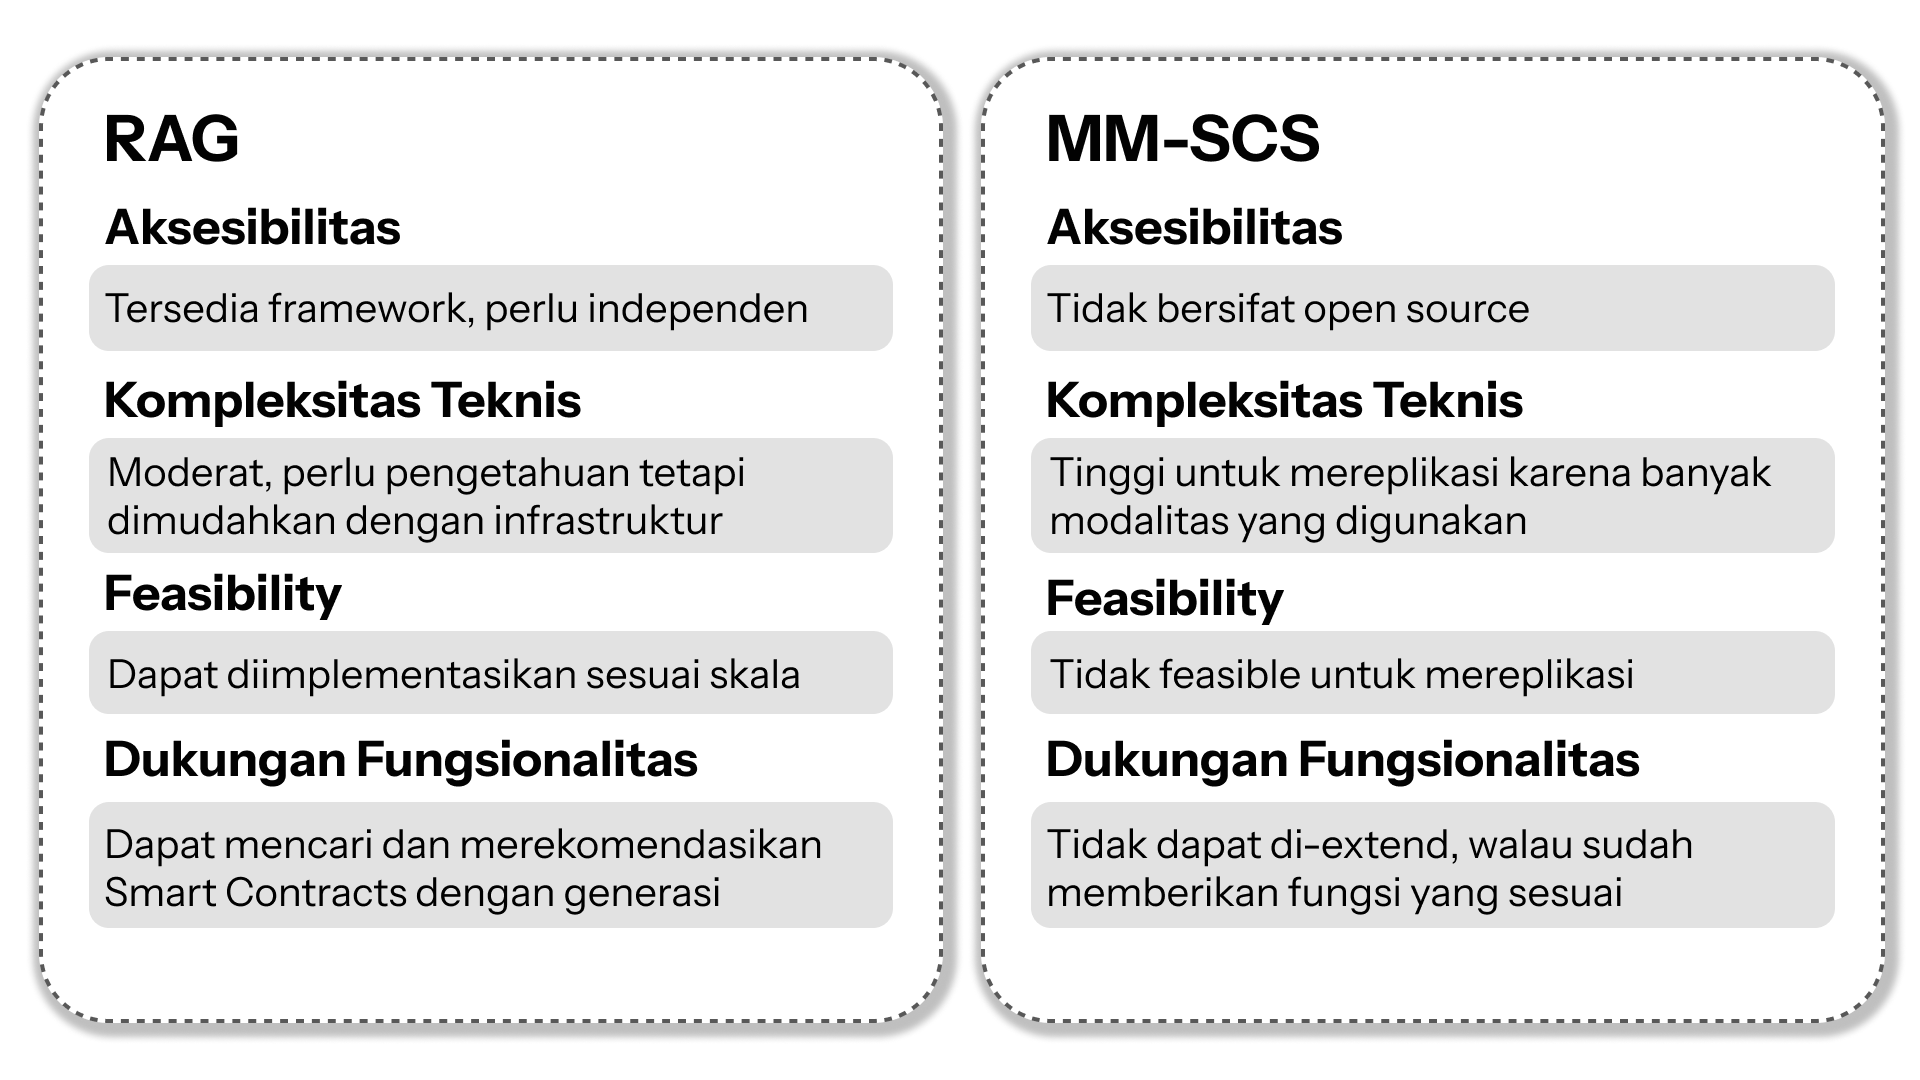
\includegraphics[width=0.9\textwidth]{resources/chapter-3/pencarian-1.png}
	\caption{Perbandingan alternatif pencarian dan rekomendasi Smart Contracts}
	\label{image:pencarian-1}
\end{figure}

\begin{figure}[ht]
	\centering
	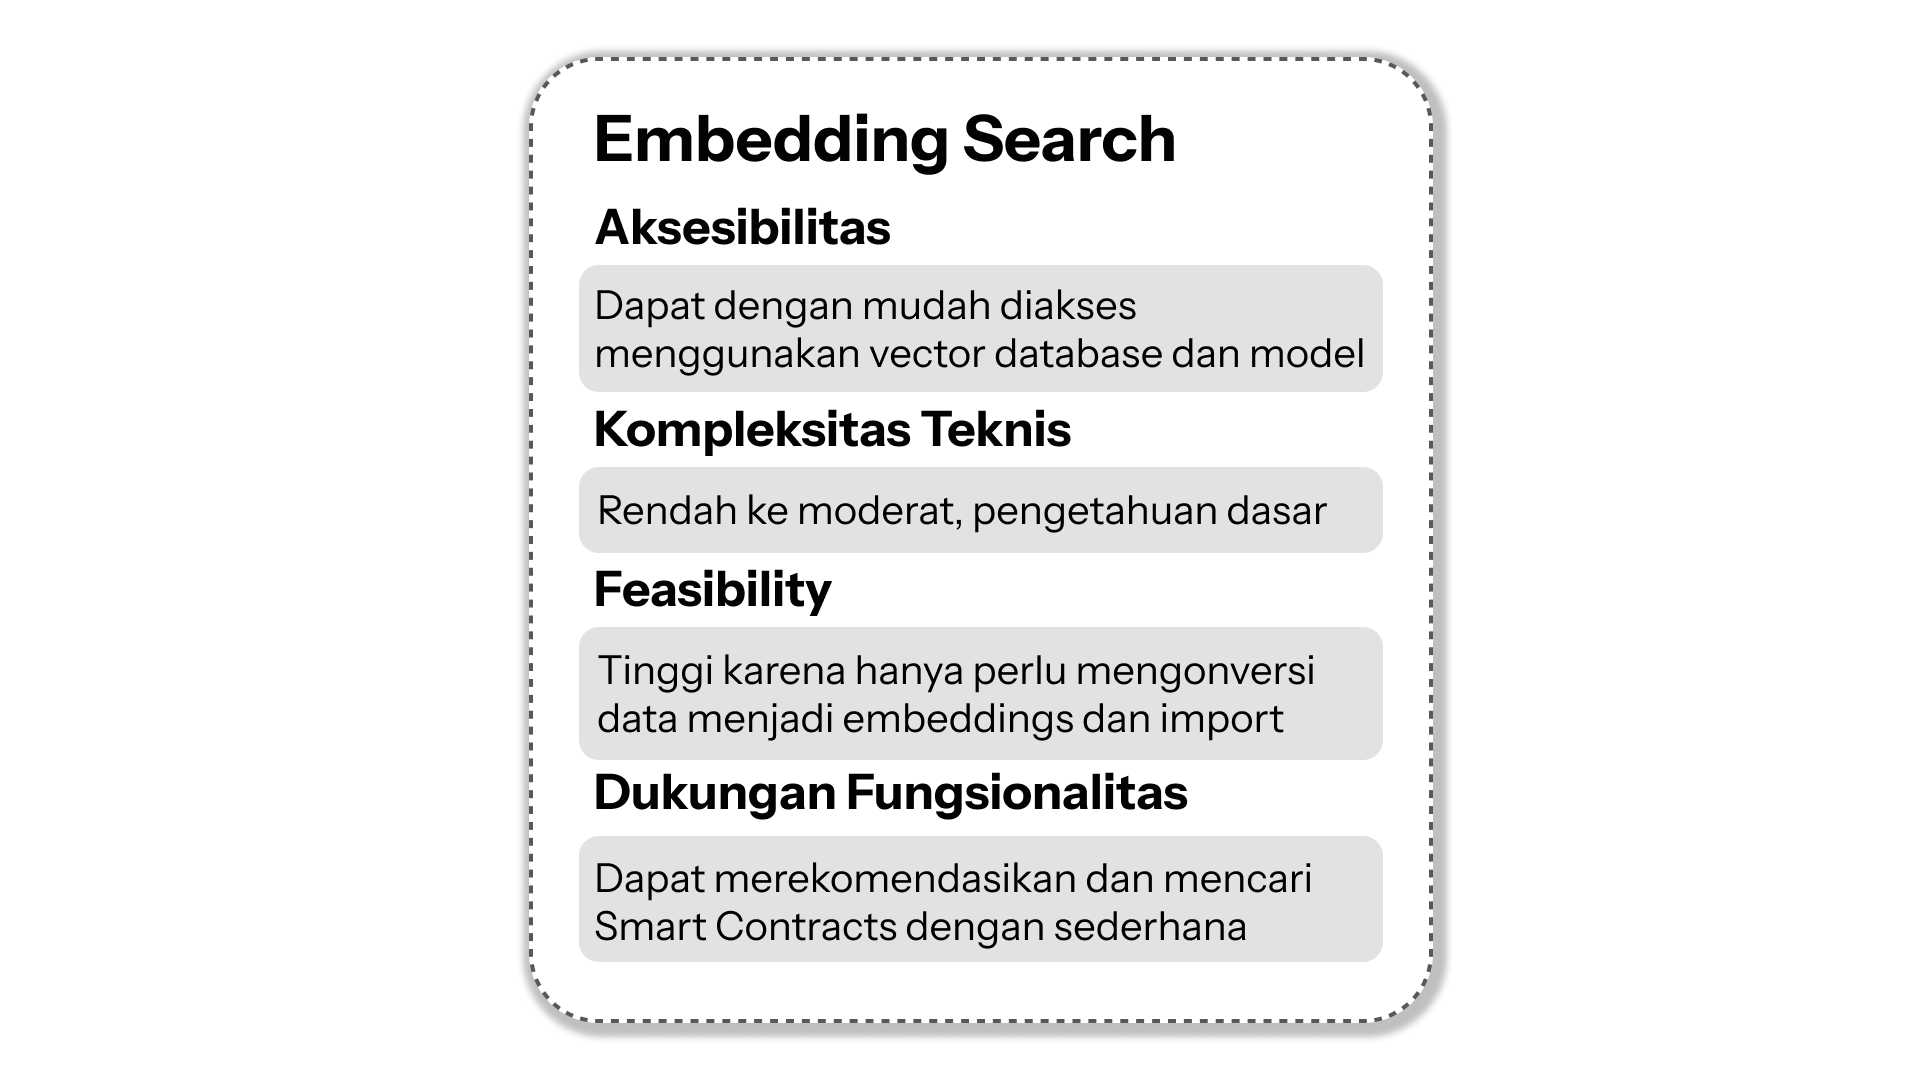
\includegraphics[width=0.9\textwidth]{resources/chapter-3/pencarian-2.png}
	\caption{Perbandingan alternatif pencarian dan rekomendasi Smart Contracts}
	\label{image:pencarian-2}
\end{figure}

Setelah data diklasifikasikan, data akan disimpan dengan format yang sesuai untuk memudahkan pencarian dan rekomendasi. Aspek skalabilitas dalam bagian ini akan digantikan dengan aspek \textit{feasibility}.

Gambar \ref{image:pencarian-1} dan \ref{image:pencarian-2} menunjukkan rangkuman perbandingan berbagai alternatif pencarian dan rekomendasi Smart Contracts. Secara rinci, berikut adalah analisis dari masing-masing alternatif:

\begin{enumerate}
	\item \textbf{Retrieval-Augmented Generation (RAG)} (Bagian \ref{sec:rag}): RAG adalah sebuah metode pipeline AI untuk menambahkan kemampuan pencarian dengan menggunakan sebuah \textit{retriever} untuk mendapatkan data dari sumber data eksternal. Secara aksesibilitas, terdapat \textit{framework} dan \textit{tools} yang dapat digunakan untuk membangun sistem berbasis RAG. Secara kompleksitas, RAG tergolong moderat karena walau membutuhkan pengetahuan terkait RAG, implementasi dari RAG dapat dimudahkan dengan infrastruktur yang sudah ada. Secara \textit{feasibility}, sistem ini dapat diimplementasikan sesuai skala yang diinginkan. Secara dukungan fungsional, RAG dapat digunakan untuk melakukan pencarian dan rekomendasi Smart Contracts lalu melakukan generasi jawaban dengan baik, walau terdapat redundansi layer generasi jika sistem hanya digunakan untuk pencarian.

	\item \textbf{Multimodal Smart Contract Search} \parencite{shi2021semantic} (Bagian \ref{subsec:semantic-code-search}): Riset ini mengusulkan sebuah sistem pencarian Smart Contracts berbasis multimodal, yang tidak hanya menggunakan teks, tetapi juga menggunakan alur kontrol (Contract Elements Dependency Graph). Meskipun hasil dari riset ini baik, sistem yang dihasilkan tidak bersifat \textit{open source} sehingga tidak dapat digunakan untuk membangun sistem di atasnya. Secara kompleksitas, untuk mereplikasi sistem ini membutuhkan kemampuan teknis yang tinggi karena dibutuhkan pemahaman dan keterampilan untuk membangun komponen-komponen di dalam \textit{framework} MM-SCS seperti modul GAT (Graph Attention Network) yang menganalisa CEDG. Secara dukungan fungsional, sistem tidak dapat di-\textit{extend}, walaupun sudah mengakomodasi untuk pendekatan semantik berbasis eksekusi kode.

	\item \textbf{Vector Embedding Search}: Vector Embedding Search adalah metode pencarian yang menggunakan representasi vektor sebagai embedding dari data yang akan dicari. Cara kerjanya adalah dengan membuat embedding dari query dan mencari kemiripan antar vektor dari query dengan data. Secara aksesibilitas, terdapat Vector Database yang dapat mengakomodasi pencarian ini. Secara kompleksitas, Vector Embedding Search tergolong rendah ke moderat karena hanya membutuhkan pengetahuan dasar tentang Vector Embeddings dan Vector Database. Secara \textit{feasibility}, tergolong tinggi karena hanya perlu mengonversi data ke dalam bentuk embeddings dan menyimpannya di dalam Vector Database. Secara dukungan fungsional, Vector Embedding Search dapat digunakan untuk melakukan pencarian dan rekomendasi Smart Contracts dengan baik dengan implementasi dan fungsionalitas sederhana.
\end{enumerate}